
\section{Reference Tracking}

The final part of the assignment requires a single policy that can both swing up
the disk from the downward position and track a reference motion around the
upright position \cite{assignment5sc28}. To address this task, the fixed-target DQN controller was
extended to a reference-conditioned DQN policy. The same learned policy is used
for both swing-up and tracking, rather than switching between separately trained
controllers. The wrapped tracking error is defined as
\begin{equation}
    e_{\mathrm{trk},k}
    =
    \mathrm{wrap}(\theta_k-\theta_{\mathrm{ref},k}),
\label{eq:tracking_error}
\end{equation}
and the input is constrained by \(u_k\in[-3,3]\) V.

The reference-conditioned DQN follows the same value-based learning principle
as the fixed-target DQN, but the state and reward are modified so that the
policy can react to the provided reference trajectory. The reward penalizes the
wrapped tracking error, excessive angular velocity, and unnecessary input
effort, while still encouraging successful swing-up. During training,
\(\epsilon\)-greedy exploration, experience replay, and a target network were
used as in the fixed-target DQN controller \cite{course5sc28,mnih2015dqn}. The increasing training return and
decreasing last-window tracking error indicated that the policy learned the
combined swing-up and tracking task.

After training, the best checkpoint was evaluated using the greedy policy.
Figure~\ref{fig:ref_dqn_eval} shows the measured angle, reference trajectory,
and wrapped tracking error. The disk is first swung up from the downward
position. During this initial transient, the tracking error is large because
the disk is still far from the reference. After the swing-up phase, the angle
approaches the reference around the upright position and the wrapped tracking
error remains close to zero.

\begin{figure}[H]
    \centering
    \begin{subfigure}[t]{0.48\linewidth}
        \centering
        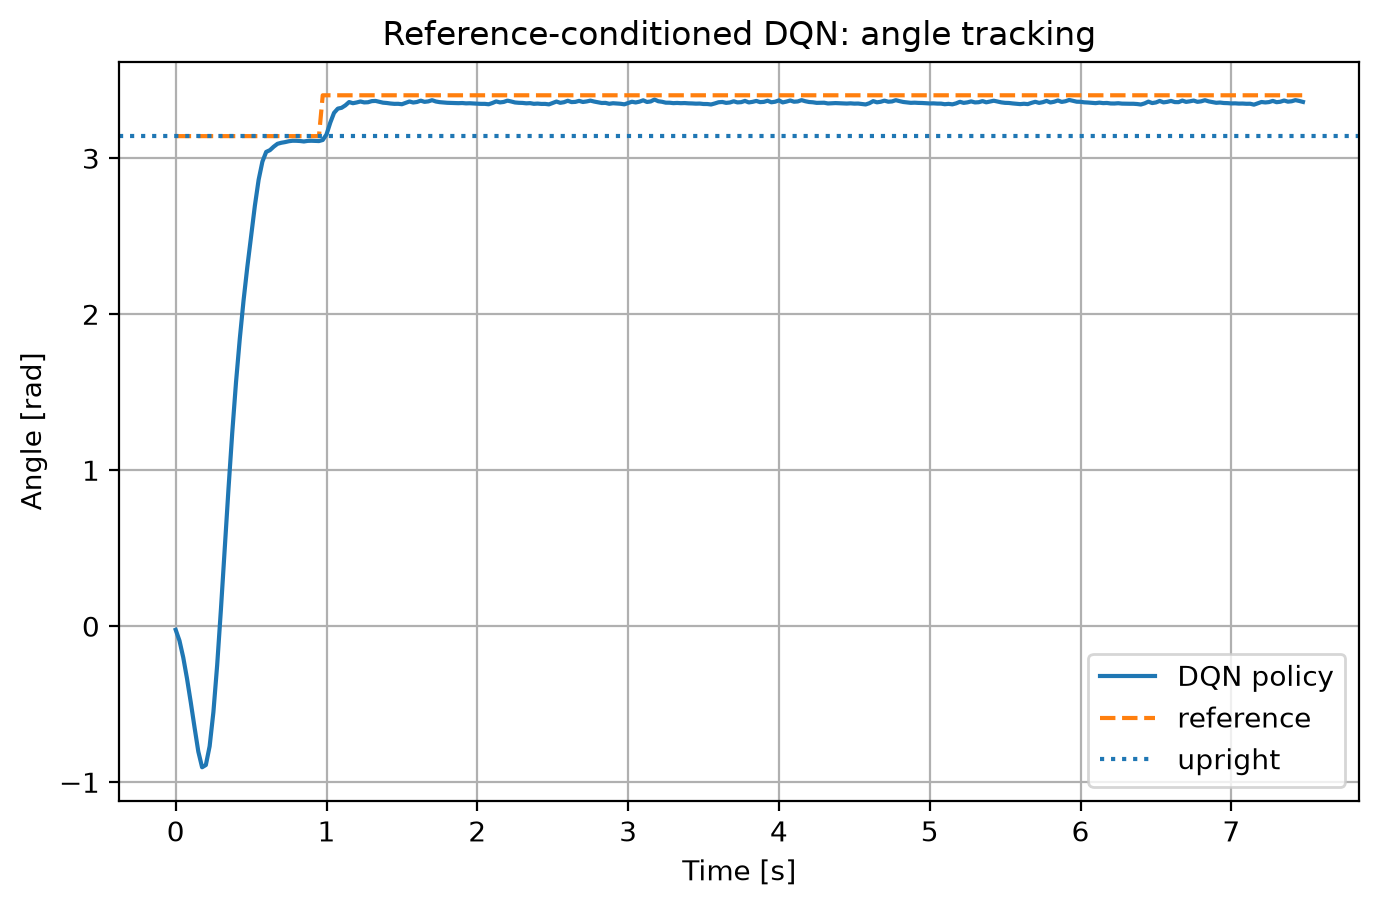
\includegraphics[width=\linewidth]{figures/ref_dqn_eval_best_theta_ref.png}
        \caption{Angle and reference.}
        \label{fig:ref_dqn_theta_ref}
    \end{subfigure}
    \hfill
    \begin{subfigure}[t]{0.48\linewidth}
        \centering
        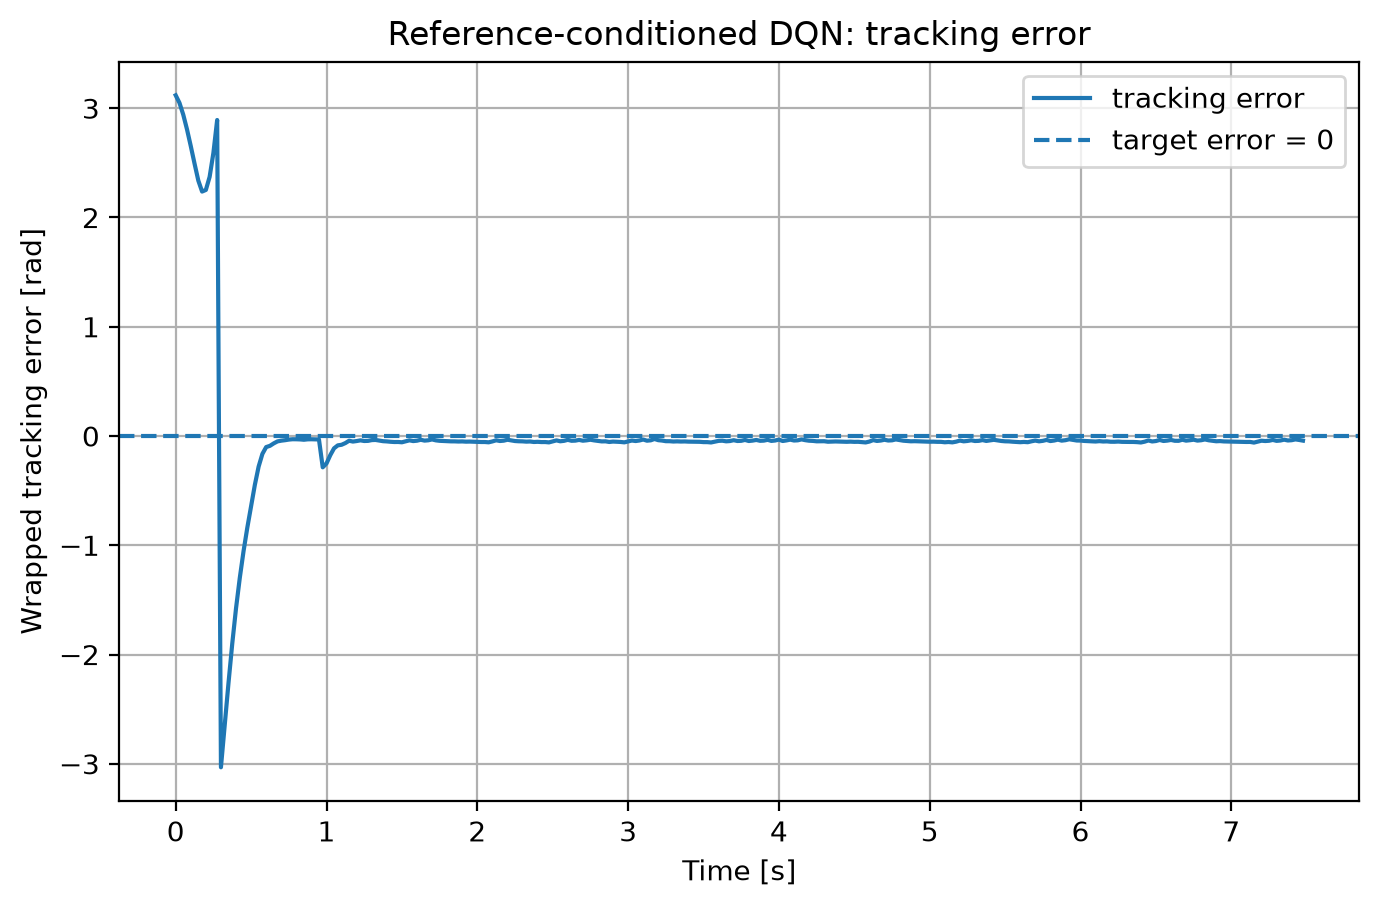
\includegraphics[width=\linewidth]{figures/ref_dqn_eval_best_error.png}
        \caption{Wrapped tracking error.}
        \label{fig:ref_dqn_tracking_error}
    \end{subfigure}
    \caption{Evaluation of the reference-conditioned DQN policy. The policy
    first swings up the disk and then tracks the reference around the upright
    region.}
    \label{fig:ref_dqn_eval}
\end{figure}

The policy was further evaluated over 20 random seeds. The results are
summarized in Table~\ref{tab:ref_dqn_results}. The reference-conditioned DQN
achieved a success rate of \(1.000\). The mean final tracking error was
\(-0.0254\) rad, the mean last-window tracking error was \(0.0310\) rad, and
the tracking ratio was \(0.9192\). These results show that the policy
consistently tracks the reference after the swing-up transient.

\begin{table}[htbp]
    \caption{Multi-seed evaluation performance of the reference-conditioned
    DQN policy.}
    \centering
    \begin{tabular}{lc}
        \toprule
        Metric & Value \\
        \midrule
        Final tracking error [rad] & $-0.0254 \pm 0.0175$ \\
        Min. abs. error [rad] & $0.0090 \pm 0.0127$ \\
        Mean abs. error [rad] & $0.1882 \pm 0.0125$ \\
        Last-window tracking error [rad] & $0.0310 \pm 0.0160$ \\
        Last-window $|\omega|$ [rad/s] & $0.3093 \pm 0.1156$ \\
        Tracking ratio & $0.9192 \pm 0.0041$ \\
        Saturation ratio & $0.1553 \pm 0.0979$ \\
        Maximum input [V] & $3.0000 \pm 0.0000$ \\
        Return & $1372.2714 \pm 6.4402$ \\
        \bottomrule
    \end{tabular}
    \label{tab:ref_dqn_results}
\end{table}

The full-rollout mean absolute error is larger than the last-window tracking
error because it includes the initial swing-up transient. Therefore, the
last-window error better reflects the steady-state tracking performance after
the disk has reached the upright region. The saturation ratio was \(0.1553\),
and the maximum input magnitude was \(3.0\) V, confirming that the voltage
constraint was satisfied but that the discrete DQN policy still used saturated
actions during part of the rollout.

Overall, the reference-conditioned DQN successfully extends the fixed-target
swing-up controller to reference tracking around the upright position using a
single learned policy. The main limitation is the switching input caused by the
discrete action representation. In addition, the current evaluation is based on
the tested reference trajectory; further tests with multiple reference signals
over the full \(\pm 15^\circ\) range would provide a more complete assessment.
